\chapter{METHODOLOGY}

\section{System Components}

The proposed system is a lightweight multimodal guardrail designed to detect jailbreak attempts in combined text-and-image inputs before they reach the protected Vision-Language Model (VLM). The methodology consists of several stages, including input routing, feature extraction, feature projection, feature fusion, classification, threshold-based decision making, and final interaction with the protected VLM.
\begin{figure}[H]  
    \centering
    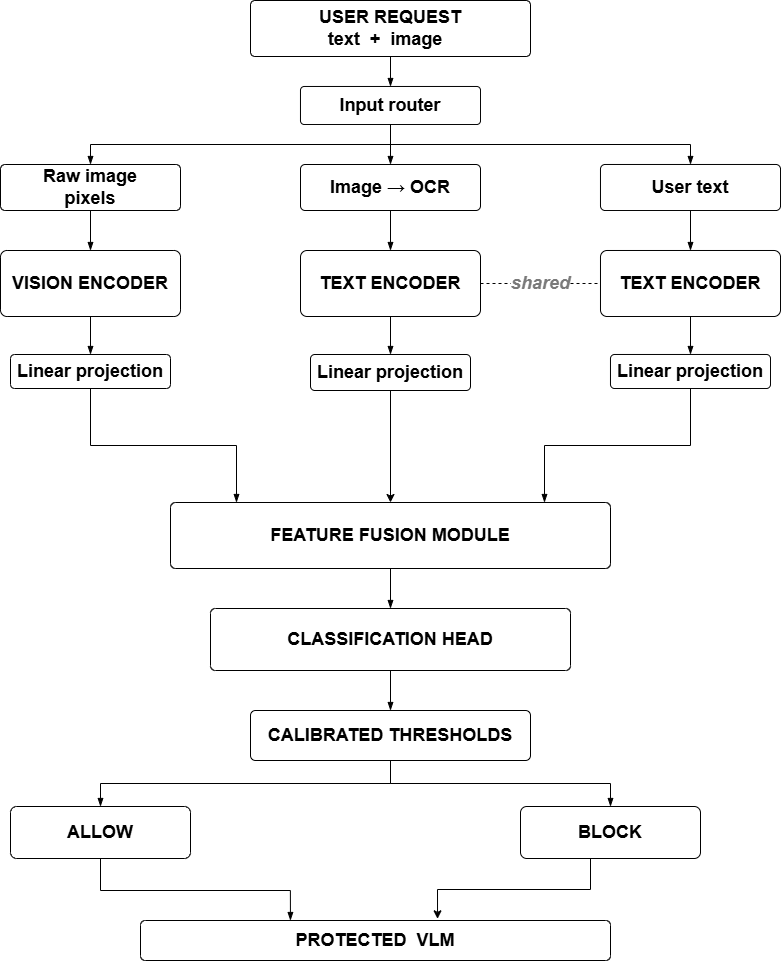
\includegraphics[width=0.8\textwidth]{Graphics/finalSystemDesign.drawio.png}
    \caption{System Design Architecture for Multimodal Guardrail}
\end{figure}


\subsection{User Request}

The system first receives a user request containing text and an image. Both modalities are considered because a jailbreak instruction may be present directly in the user's text or hidden within the image.

\subsection{Input Router}

The input router receives the complete user request and separates it into three branches: raw image pixels, text extracted from the image using Optical Character Recognition (OCR), and the original user text. This separation allows the system to independently analyze the visual and textual information.

\subsection{Raw Image Processing}

The raw image pixels are directly passed to the vision encoder. This branch captures visual information from the image, including visual patterns, objects, layouts, and text-like features that may not be successfully extracted by OCR.

\subsection{Vision Encoder}

The raw image is processed using a vision encoder . The encoder converts the image into a numerical feature representation. These features contain information about the visual content of the input and are later used by the feature fusion module for jailbreak detection.

\subsection{Image-to-OCR Processing}

The image is also passed through an Optical Character Recognition (OCR) module to extract text present inside the image. This is important for detecting typographic injection attacks, where a malicious instruction is embedded as text within an image.

\subsection{OCR Text Encoder}

The text extracted by OCR is passed to a text encoder. The text encoder converts the extracted text into a numerical feature representation. These features provide semantic information about the text contained in the image.

\subsection{User Text Encoder}

The original user text is processed using text encoder. The encoder converts the user's textual request into a feature representation. The same encoder weights are shared between the OCR text and user text branches so that the system can process language consistently regardless of its source.

\subsection{Linear Projection}

The outputs of the vision and text encoders may have different dimensions. Therefore, linear projection layers are used to transform the extracted features into a common feature dimension. In the proposed architecture, the features are projected into a shared dimension.

This common representation allows the visual features, OCR text features, and user text features to be combined effectively in the feature fusion module.

\subsection{Classification Head}

The fused multimodal representation is passed to a classification head. The classification head is a neural network that produces a jailbreak risk score representing the likelihood that the input contains a malicious or jailbreak attempt.

For example, a lower risk score represents a safer input, while a higher risk score indicates a potentially malicious input.
\subsection{Feature Fusion}

\begin{figure}[H]
    \centering
    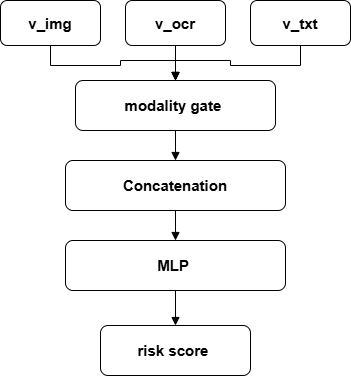
\includegraphics[width=0.7\textwidth]{Graphics/fusionimage.png}
    \caption{Feature Fusion Module Architecture}
\end{figure}

The baseline feature-fusion approach takes the feature representations from the image, OCR, and textual modalities as inputs \cite{hua2026rethinking}. The image representation captures visual information, the OCR representation captures text extracted from the image, and the textual representation captures information from the input prompt or request.

The three modality representations are first passed through a modality gating mechanism. The gate learns the relative importance of each modality and assigns appropriate weights to their corresponding feature representations. This allows the model to emphasize more informative modalities while reducing the influence of less relevant ones.

After the gating process, the resulting modality representations are concatenated to form a unified multimodal feature representation. This combined representation contains information from the image, OCR, and textual modalities and provides a common representation for subsequent processing.

The concatenated representation is then passed through a multilayer perceptron (MLP). The MLP progressively transforms the fused representation into a compact feature representation while learning interactions among the different modalities. The resulting representation is finally used to produce the risk score of the input.


\subsection{Calibrated Thresholds}

The risk score is passed through calibrated decision thresholds. Two thresholds are used to divide the risk score into different decision regions. Based on the obtained risk score, the input is classified as \textit{Allow} or \textit{Block}.

\subsection{Allow Decision}

If the risk score is below the lower threshold, the input is classified as \textit{Allow}. The request is considered sufficiently safe and is forwarded to the protected Vision-Language Model for further processing.

\subsection{Block Decision}

If the risk score is above the blocking threshold, the input is classified as \textit{Block}. The request is considered potentially harmful or malicious and is rejected by the guardrail without being forwarded to the protected Vision-Language Model.

\subsection{Protected Vision-Language Model}

The protected VLM is the downstream model that processes the requests accepted by the guardrail. The guardrail acts as an additional security layer between the user and the VLM, preventing potentially malicious multimodal inputs from directly reaching the model.
